\documentclass[11pt,letterpaper]{article}
\usepackage{fullpage}

\usepackage[english]{babel}
\usepackage[utf8]{inputenc}
\usepackage{amsmath}
\usepackage{graphicx}
\usepackage[hidelinks]{hyperref}
\usepackage{float}
\usepackage{amsfonts}
\usepackage{algorithm,algpseudocode}
\usepackage{pdfpages}
             
\graphicspath{{../results}}

\begin{document} 

\title{New Experiments}
\maketitle


\section*{More Complex Instances}
We consider the same instances as before, but we consider $K = 10$ instead of $K = 3$. Previously we had conjectured that increasing $K$ only changes the time it takes to learn, but now we want to test if difficulty to learn the best arm can impact what happens in competition. Why would we think this should happen? There are two potentially counteracting effects one can think of:
\begin{enumerate}
\item Making the learning problem harder can benefit better algorithms in the long-run since they'll be more likely to identify the best arm than the worse algorithms and thus we expect there to be a bigger difference in the reputation scores between a good algorithm and a bad algorithm
\item Making the learning problem harder also forces the better algorithms to engage in more sub-optimal exploration which could have perverse short-run effects on reputation.
\end{enumerate}

We summarize the results for each instance and comment on the difference from the $K=3$ case:
\begin{enumerate}
\item Needle in Haystack:
\begin{enumerate}
\item HMR / SM: The results are roughly the same. $TS > DEG > DG$
\item HM: In $K=3$, we had that the results were effectively 50/50 between TS and DEG/DG. However, with $K=10$, we see that TS wins by a lot.
\end{enumerate}
\item Uniform:
\begin{enumerate}
\item HMR/SM: The results are for the most part qualitatively the same. The one difference is that for $K = 10$ we see that $DEG > DG$ slightly more clearly.
\item HM: The results are also qualitatively similar, with no algorithm clearly dominating.
\end{enumerate}
\item Heavy Tail:
\begin{enumerate}
\item HMR/SM: The results are starker than with $K = 3$ arms with TS dominating DEG and DG by a lot. However, we no longer see that $DG > DEG$ as we did in $K = 3$
\item HM: The results here are starker than with $K = 3$ arms, with DEG and DG dominating TS more than in the $K = 3$ case. 
\end{enumerate}
\end{enumerate}
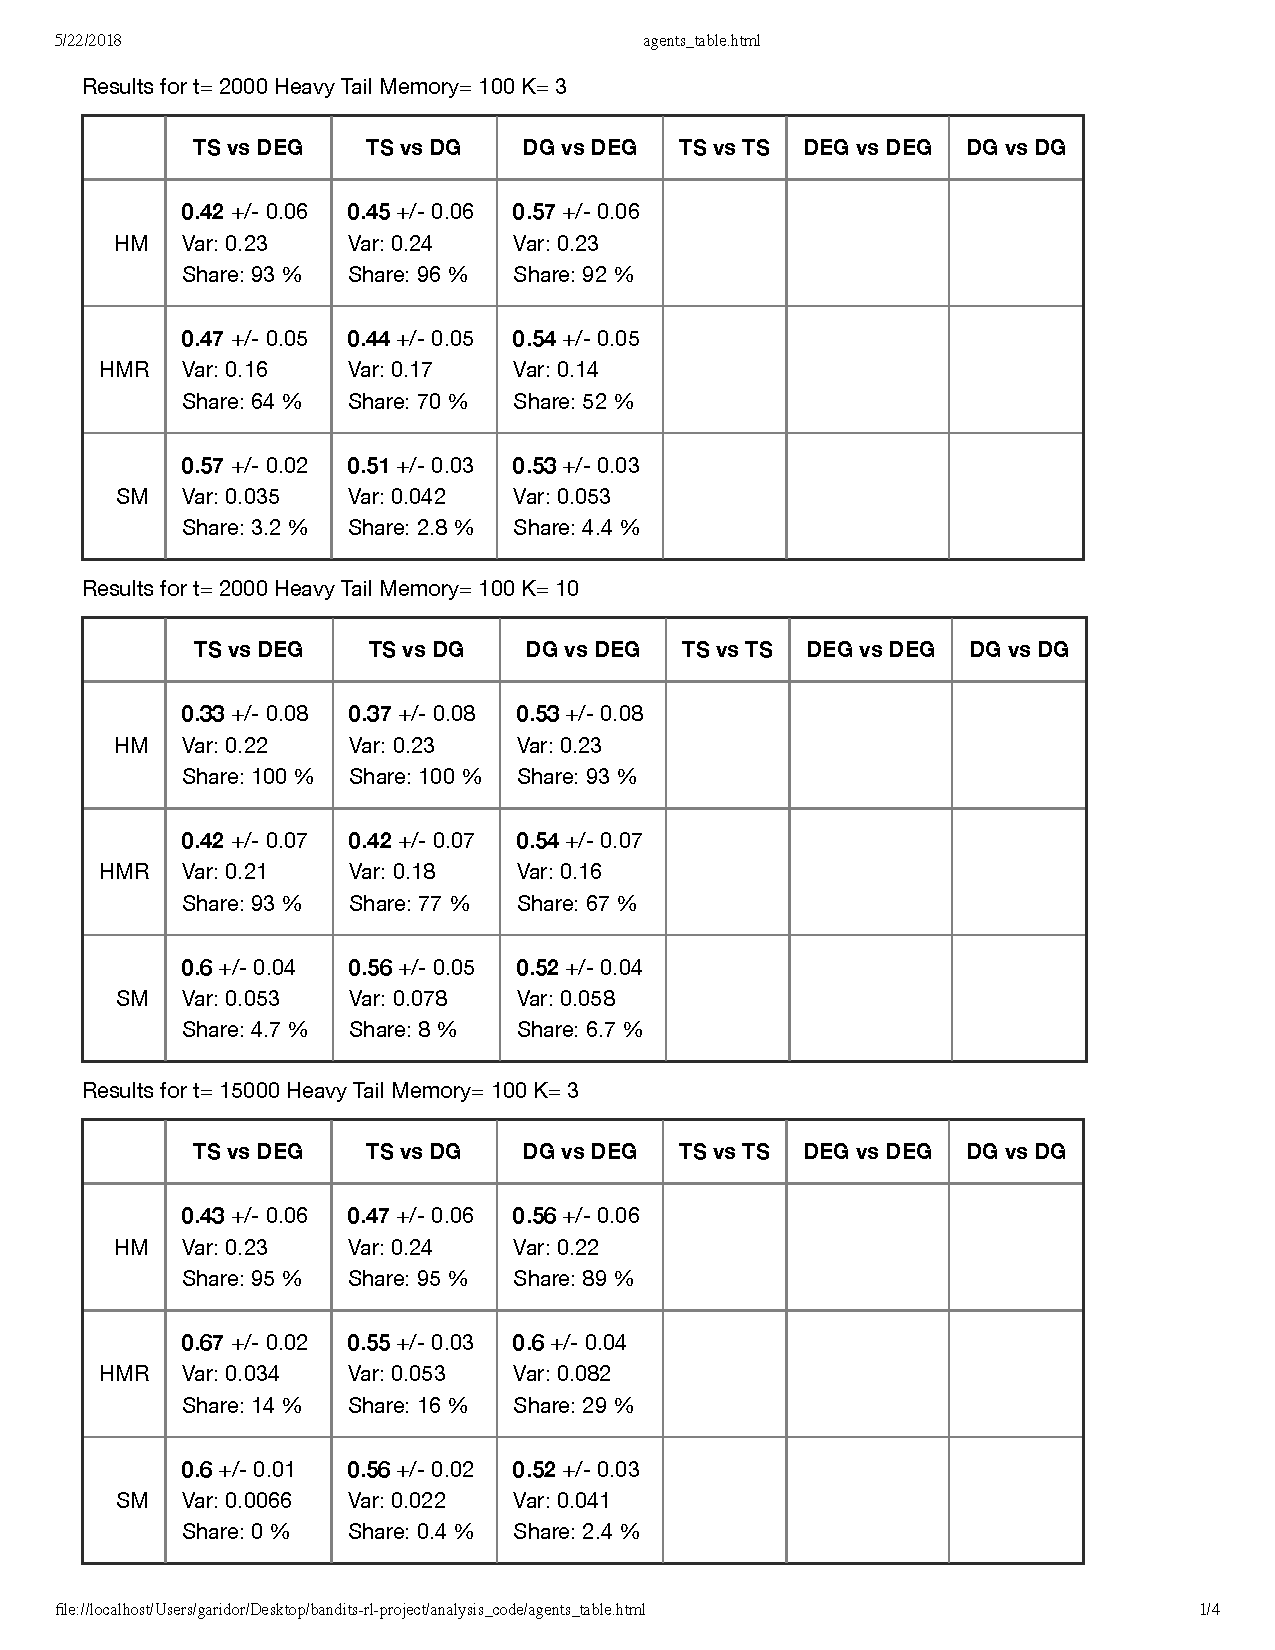
\includepdf[pages={-}]{many_arms_vs_few_arms}


\section*{Information vs Reputation - Incumbent}

The following tables contain three separate runs of the incumbent experiment (the realizations are different each time, but we should change this in future runs). The first is the one we have looked at before where one of the principals gets 200 free observations. In the second we artificially eliminate the reputation gain of the incumbent upon the entrant entering. In the third we artificially eliminate the information gain of the incumbent upon the entrant entering. Thus, the overall goal here is to ask what the effect reputation and information have individually as barriers to entry for learning.

Overall, the results are as follows:
\begin{enumerate}
\item The effect of reputation in HardMax seems to be relatively large for the incumbent. Looking at the Info table with the HardMax response function shows that the entrant gets a significant amount of the market back when the reputation gain is erased. When the information gain is erased, with HardMax the incumbent doesn't lose much market share. It appears somewhat similar in HardMaxWithRandom, but the difference is not so stark.
\item I am not sure what to make of the SoftMax case. It seems that losing reputation and information can actually \textit{benefit} the incumbent. I can't think of why this would make any sense, so I'm going to rerun these again using the same realizations. I did not record the parametrization for SoftMax during each of the runs, so it is possible that this is why we see these results. As a result, take the SoftMax results with a grain of salt until I re-run this.
\end{enumerate}


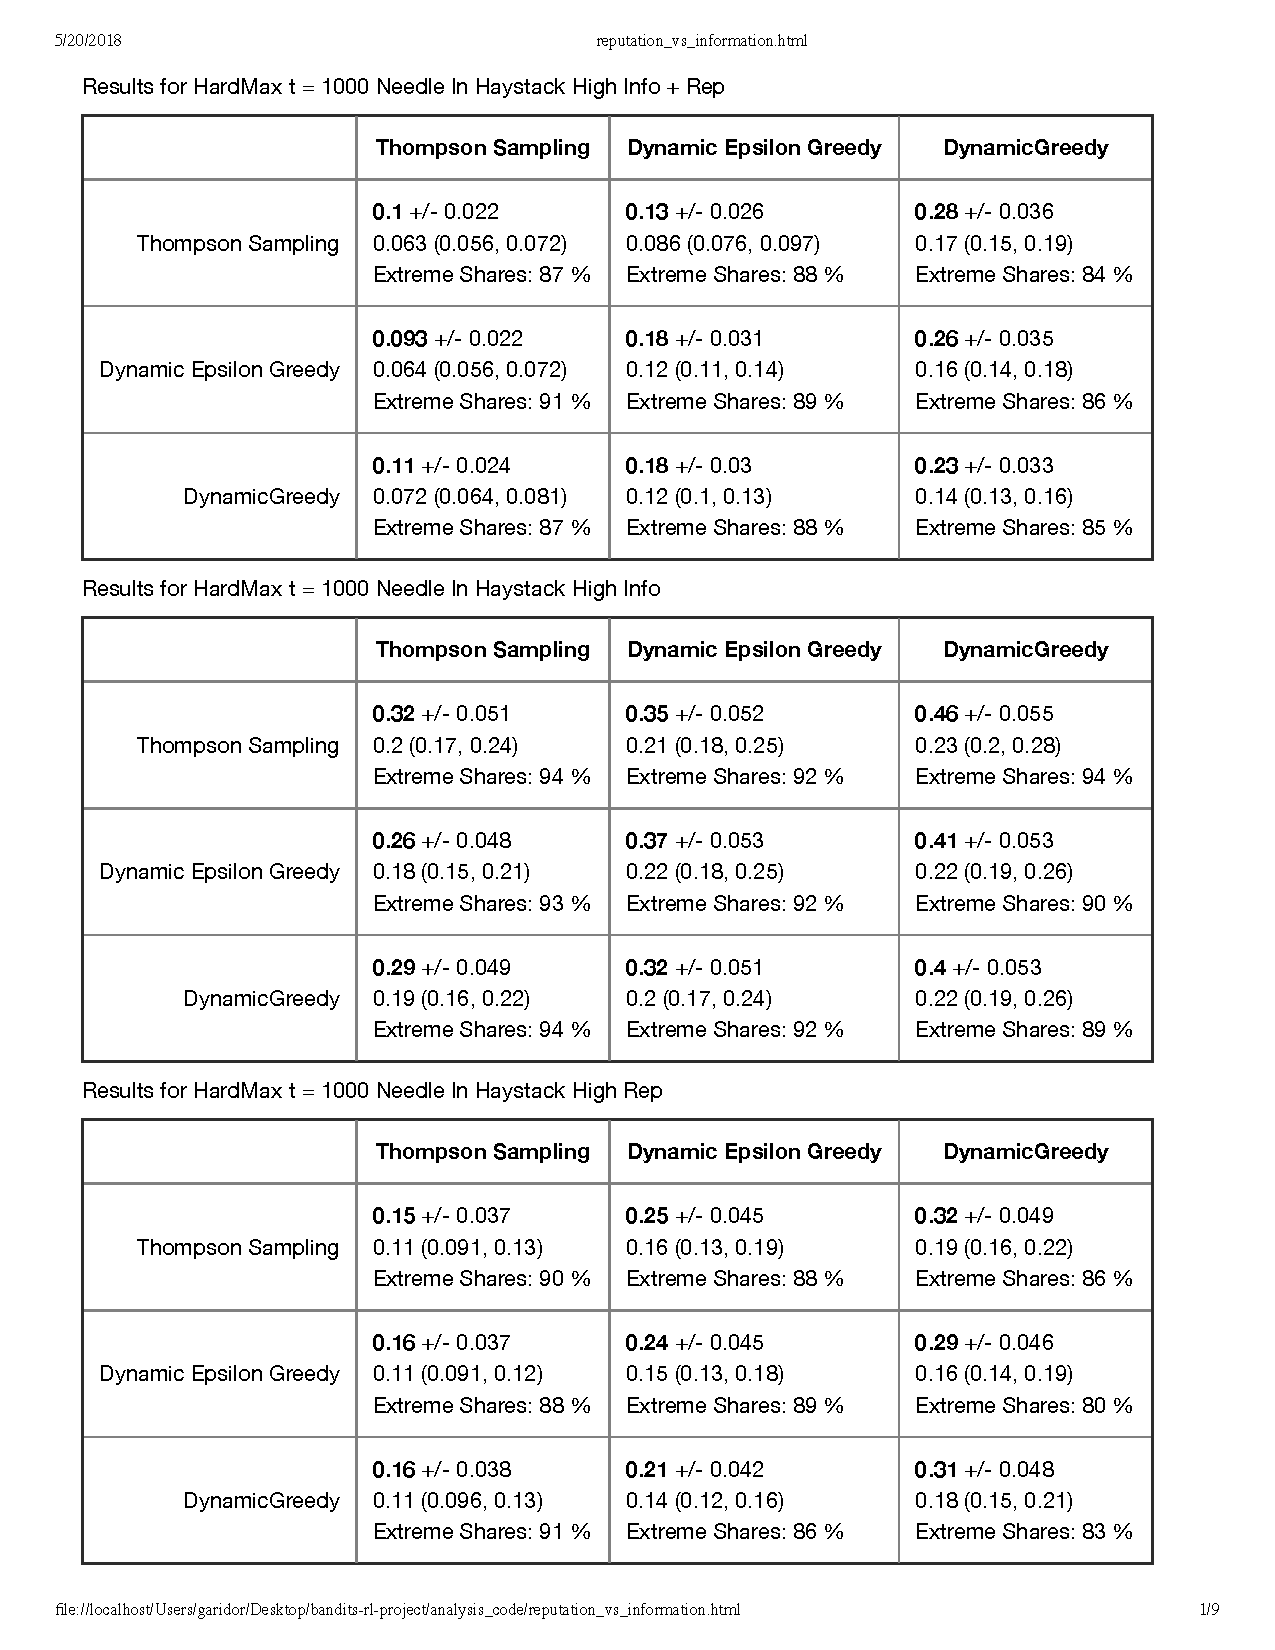
\includepdf[pages={-}]{reputation_vs_information}

\end{document}
